\chapter{ADC} \label{sec:ADC_bilag}
\section{Opsætning}
I dette afsnit beskrives hvordan ADC'en er opsat. Der fokuseres på de parametre, der er ændret og tilpasset i forhold til dette projekt.

\begin{figure}[H]
	\centering
	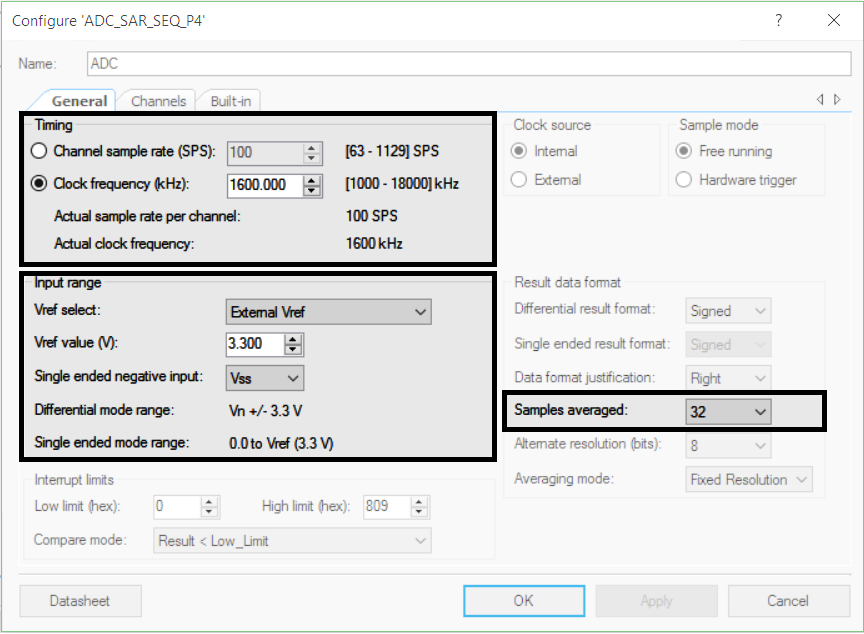
\includegraphics[width=0.5\textwidth]{figures/ADC_instillinger_edit.png}
	\caption{ADC's generelle indstillinger, hvor de fremhævede områder viser parametre, der er relevante for dette projekt. Øverste blok til venstre viser instillingsmuligheder for samplings- og clockfrekvens, samt de reelle frekvenser. Nederste blok til venstre viser instillinger for ADC'ens arbejdsområde i forhold til single ended og differential måling. Blokken til højere viser antallet af samples fortaget til at give en gennemsnitlig sample.}
	\label{fig:ADC_GeneralTab}
\end{figure}

\subsection{Bestemmelse af samplingsfrekvens}
Det markerede område øverst til venstre på \autoref{fig:ADC_GeneralTab}, viser indstillingerne for ADC'ens samplingsfrekvens, samt clock frekvens. Ved indstilling af disse frekvenser udregnes en reel samplings- og clockfrekvens. De reelle frekvenser kan variere grundet andre parametre som antal af kanaler, konverteringstid, mm. Yderligere parametre kan findes i databladet for ADC'en. 

I dette projekt opnåes en samplingsfrekvens på $100~Hz$ ved at definere en clockfrekvens på $1600~kHz$ samt ved at justere konverteringstiden af kanalerne, der ses på \autoref{fig:ADC_KanalTab}. Hertil er der pålagt en forsinkelse, således en konverteringstid på $3,32~ms$ per kanal opnås. Dette giver en konverteringstid på $9,96~ms$ for de 3 kanaler, hvilket konfigurationen af ADC'en oplyser som en samplingsfrekvens på $100~Hz$. 

\begin{figure}[H]
	\centering 
	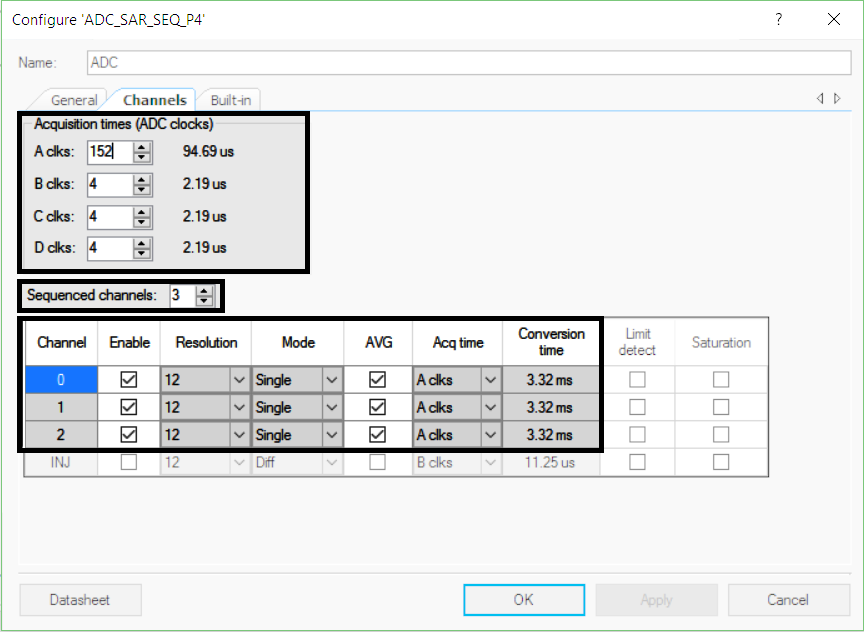
\includegraphics[width=0.5\textwidth]{figures/ADC_instillinger2_edit.png}
	\caption{Indstillinger for de enkelte inputs til ADC'en. Øverste blok viser indstillingsmuligheder for 4 ADC-clocks, der definerer konverteringstiden for kanalerne. Miderste blok viser antallet af kanaler, der defineres. Nederste blok viser indstillingsmuligheder og konvertieringstid for de enkelte kanaler.}
	\label{fig:ADC_KanalTab}
\end{figure}

\subsection{Arbejdsområde for ADC}
Det markerede område nederst til venstre på \autoref{fig:ADC_GeneralTab}, viser indstillingerne for ADC'ens arbejdsområde. Vref definerer størrelsen af arbejdsområdet, hvortil en ekstern reference er valgt. Denne reference sættes til at være identisk med mikrokontrollerens forsyning til acceleromterne på $3,3~V$. Det negative input for single ended målinger sættes til Vss (jord). Dette giver et arbejdsområde for single ended målinger på $0,0~V - 3,3~V$. Da det negative input tilsluttes jord, falder opløsningen $1~bit$, da der ikke kan forekomme negative udslag i arbejdsområdet. 

\subsection{Gennemsnits samples}
Det markerede område til højre på \autoref{fig:ADC_GeneralTab} er indstillingen for, hvor mange samples der anvendes for hver af kanalerne til at repræsentere én konverteret sample. Der benyttes derfor 32 samples til at udregne én gennemsnits-sample, som er den sample, der benyttes i systemet. Dette gøres gældende for kanaler, hvor 'AVG' er afkrydset, som det ses af nederste blok i \autoref{fig:ADC_KanalTab}. Dette er implementeret, da samplingsfrekvensen på $100~Hz$ opretholdes, samt at flere samples, der tilsammen udgør én gennemsnitlig sample, repræsenterer den samplede værdi bedre end én enkelt sample. 





